\section{Cấu hình máy chủ và Môi trường hệ thống}
\label{sec:cau-hinh-server}

Để vận hành quy trình CI/CD hoàn chỉnh, nhóm đã triển khai một máy chủ riêng biệt trên nền tảng điện toán đám mây.

\subsection{Khởi tạo máy chủ trên AWS (EC2)}
Nhóm sử dụng dịch vụ Amazon EC2 để tạo máy chủ với các thông số sau:
\begin{itemize}[noitemsep]
    \item \textbf{Hệ điều hành}: Ubuntu Server 24.04 LTS (Hỗ trợ tốt nhất cho Docker)
    \item \textbf{Instance Type}: \texttt{t3.small} (2 vCPU, 2GB RAM).
    \item \textbf{Bộ nhớ mở rộng (Swap Memory)}: Cấu hình 4GB Swap để tránh tình trạng tràn bộ nhớ (Out-of-memory) khi SonarQube và Jenkins chạy đồng thời.
\end{itemize}

\begin{figure}[H]
    \centering
    % CHỈ DẪN ẢNH: Thả ảnh 01-aws-ec2-instances-list.png vào thư mục img/
    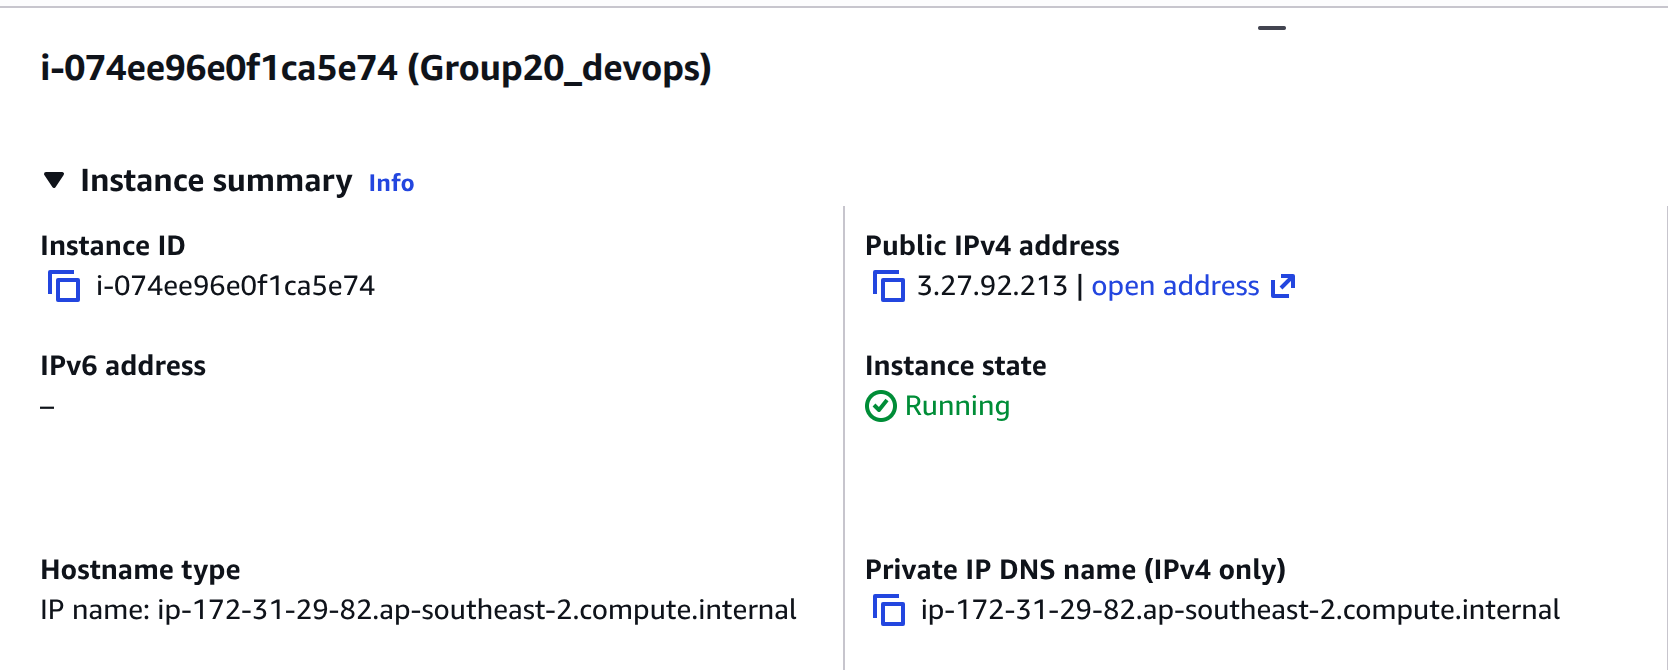
\includegraphics[width=0.9\textwidth]{img/01-aws-ec2-instances-list.png}
    \caption{Danh sách các máy chủ EC2 phục vụ hệ thống CI/CD}
\end{figure}

Trên AWS Console, nhóm tạo một Security Group và mở các cổng mạng thiết yếu (22, 8080, 9000, 50000).

\begin{figure}[H]
    \centering
    % CHỈ DẪN ẢNH: Thả ảnh 02-aws-security-group-rules.png vào thư mục img/
    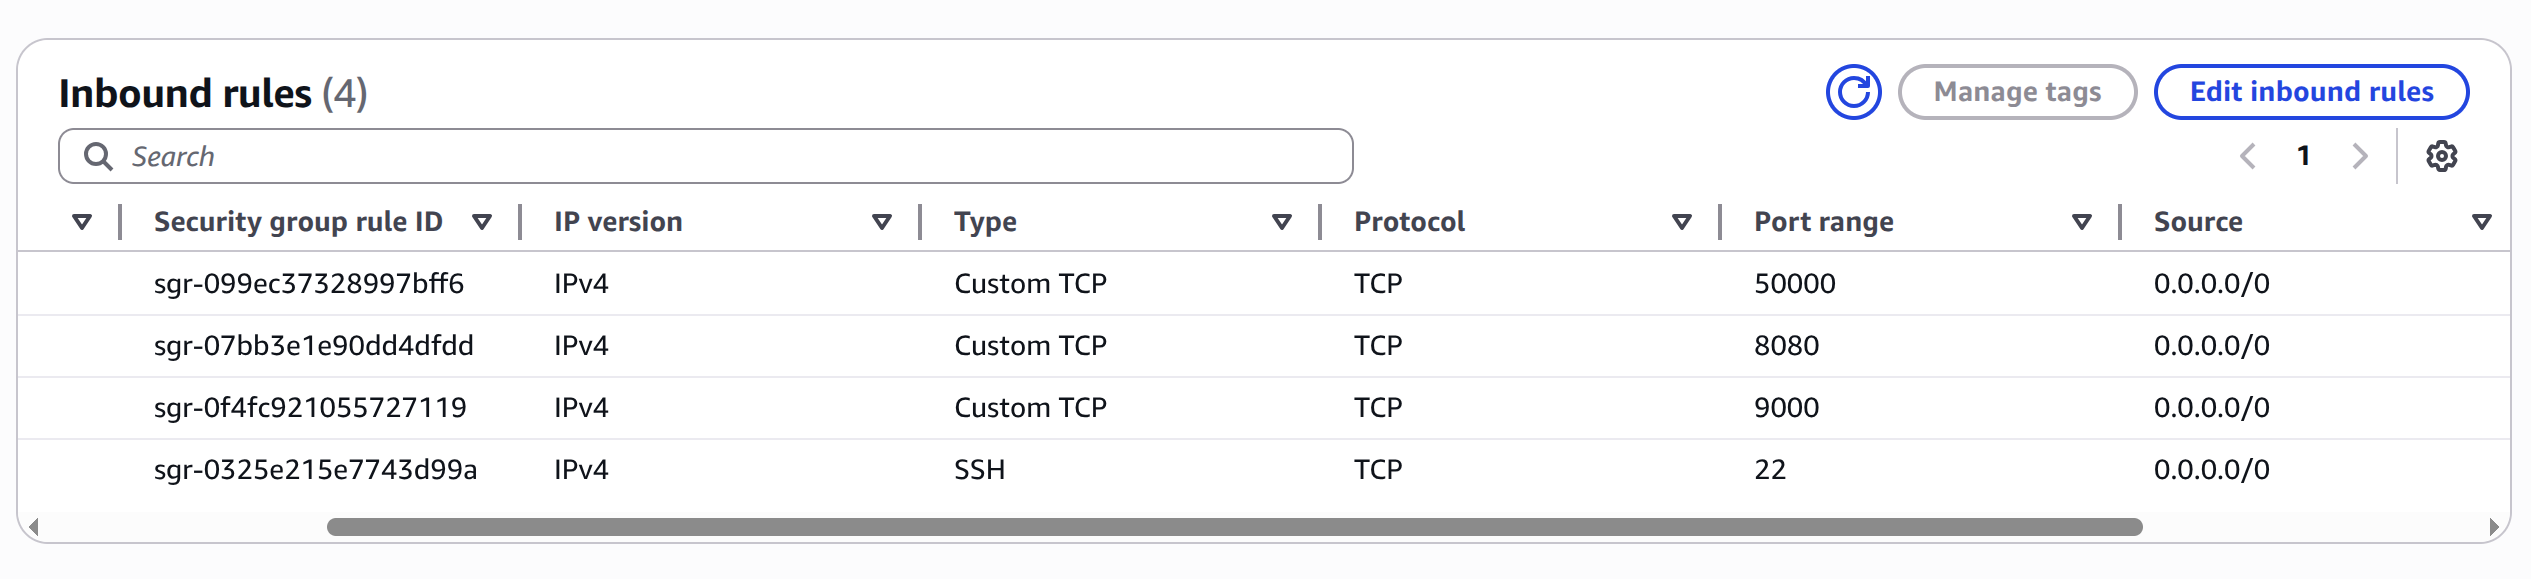
\includegraphics[width=0.9\textwidth]{img/02-aws-security-group-rules.png}
    \caption{Thiết lập quy tắc Inbound rules của Security Group}
\end{figure}

\subsection{Cài đặt và Quản trị môi trường Docker}
Dự án sử dụng công nghệ Container để cô lập môi trường và dễ dàng quản lý dịch vụ.

\textbf{Cài đặt Docker Engine}: Nhóm tiến hành cài đặt các gói \texttt{docker.io} và \texttt{docker-compose} trên nền tảng Ubuntu.

\begin{lstlisting}[language=bash, caption={Cài đặt Docker trên Ubuntu Server}]
# Cap nhat he thong
sudo apt update && sudo apt upgrade -y

# Cai dat Docker Engine
sudo apt install docker.io -y
sudo systemctl start docker
sudo systemctl enable docker

# Cap quyen chay Docker khong can sudo
sudo usermod -aG docker $USER

# Cai dat Docker Compose
sudo apt install docker-compose -y
\end{lstlisting}

\textbf{Thiết lập cấu hình triển khai (Docker Compose)}: Thay vì cài đặt rời rạc, dự án sử dụng Docker Compose để quản lý tập trung Jenkins và SonarQube.

\begin{lstlisting}[language=make, caption={Tệp cấu hình docker-compose.yml tiêu chuẩn}]
version: '3.8'
services:
  jenkins:
    image: jenkins/jenkins:lts
    container_name: jenkins
    ports:
      - "8080:8080"
      - "50000:50000"
    volumes:
      - jenkins_home:/var/jenkins_home
      - /var/run/docker.sock:/var/run/docker.sock
    restart: always

  sonarqube:
    image: sonarqube:lts-community
    container_name: sonarqube
    ports:
      - "9000:9000"
    environment:
      - SONAR_ES_BOOTSTRAP_CHECKS_DISABLE=true
    volumes:
      - sonarqube_data:/opt/sonarqube/data
    restart: always

volumes:
  jenkins_home:
  sonarqube_data:
\end{lstlisting}

\textbf{Quản trị bằng Docker CLI}: Thay vì cài đặt truyền thống, việc tương tác với dịch vụ được thực hiện qua các lệnh thực thi trực tiếp vào Container.

\textbf{Lấy mật khẩu Jenkins}: Sử dụng lệnh sau để lấy mã unlock hệ thống ban đầu:
\begin{lstlisting}[language=bash]
docker exec jenkins cat /var/jenkins_home/secrets/initialAdminPassword
\end{lstlisting}

\textbf{Kiểm tra trạng thái}: Sử dụng lệnh sau để xác nhận các container \texttt{jenkins} và \texttt{sonarqube} đang vận hành ổn định:
\begin{lstlisting}[language=bash]
docker ps
\end{lstlisting}

\begin{figure}[H]
    \centering
    % CHỈ DẪN ẢNH: Thả ảnh 03-docker-ps-status.png vào thư mục img/
    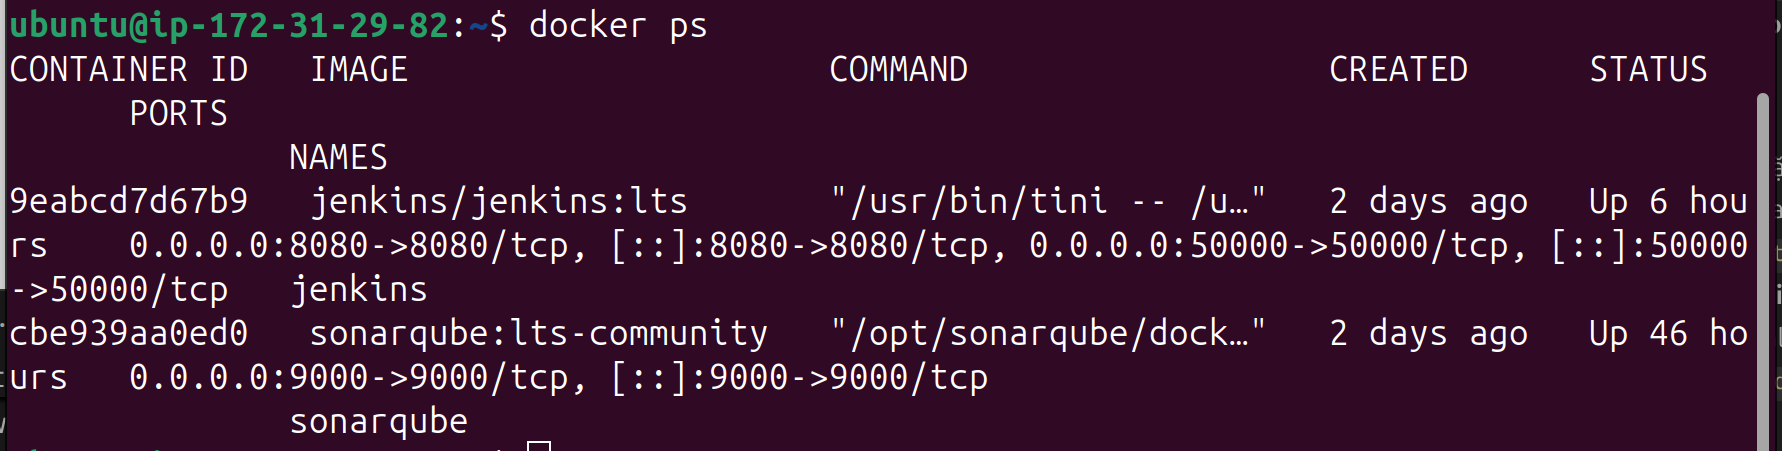
\includegraphics[width=0.9\textwidth]{img/03-docker-ps-status.png}
    \caption{Danh sách các container dịch vụ đang hoạt động ổn định}
\end{figure}

\subsection{Cấu hình tích hợp hệ thống (System Integration)}
Thiết lập luồng giao tiếp tự động giữa GitHub, Jenkins và SonarQube.

\textbf{GitHub Webhook}: Cấu hình Webhook trên Repository để gửi tín hiệu tới Jenkins mỗi khi có sự kiện Push hoặc Pull Request.

\begin{figure}[H]
    \centering
    % CHỈ DẪN ẢNH: Thả ảnh 05-github-webhook-config.png vào thư mục img/
    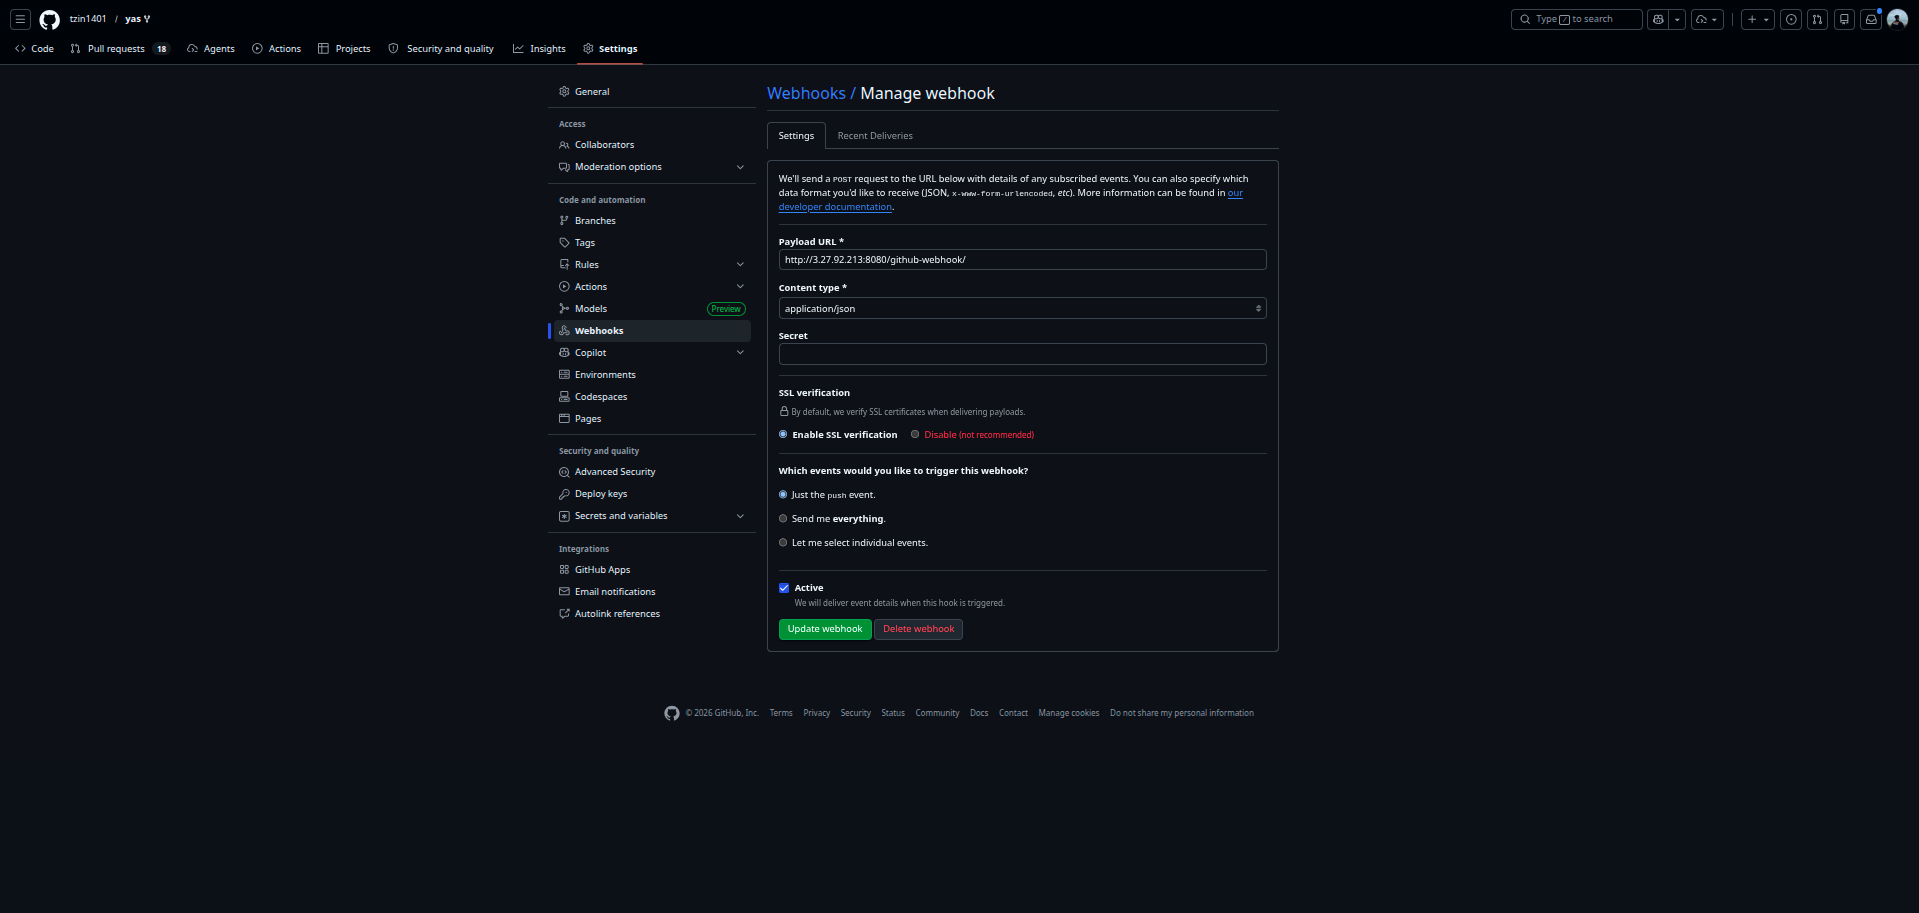
\includegraphics[width=0.9\textwidth]{img/03-github-webhook-list1.png}
    \caption{URL Webhook trên GitHub có dấu tích xanh (Active)}
\end{figure}

\textbf{SonarQube Webhook}: Cấu hình Webhook ngược từ SonarQube về Jenkins (\texttt{http://<IP-Jenkins>:8080/sonarqube-webhook/}) để trả kết quả Quality Gate.

\begin{figure}[H]
    \centering
    % CHỈ DẪN ẢNH: Thả ảnh 06-sonarqube-webhook-config.png vào thư mục img/
    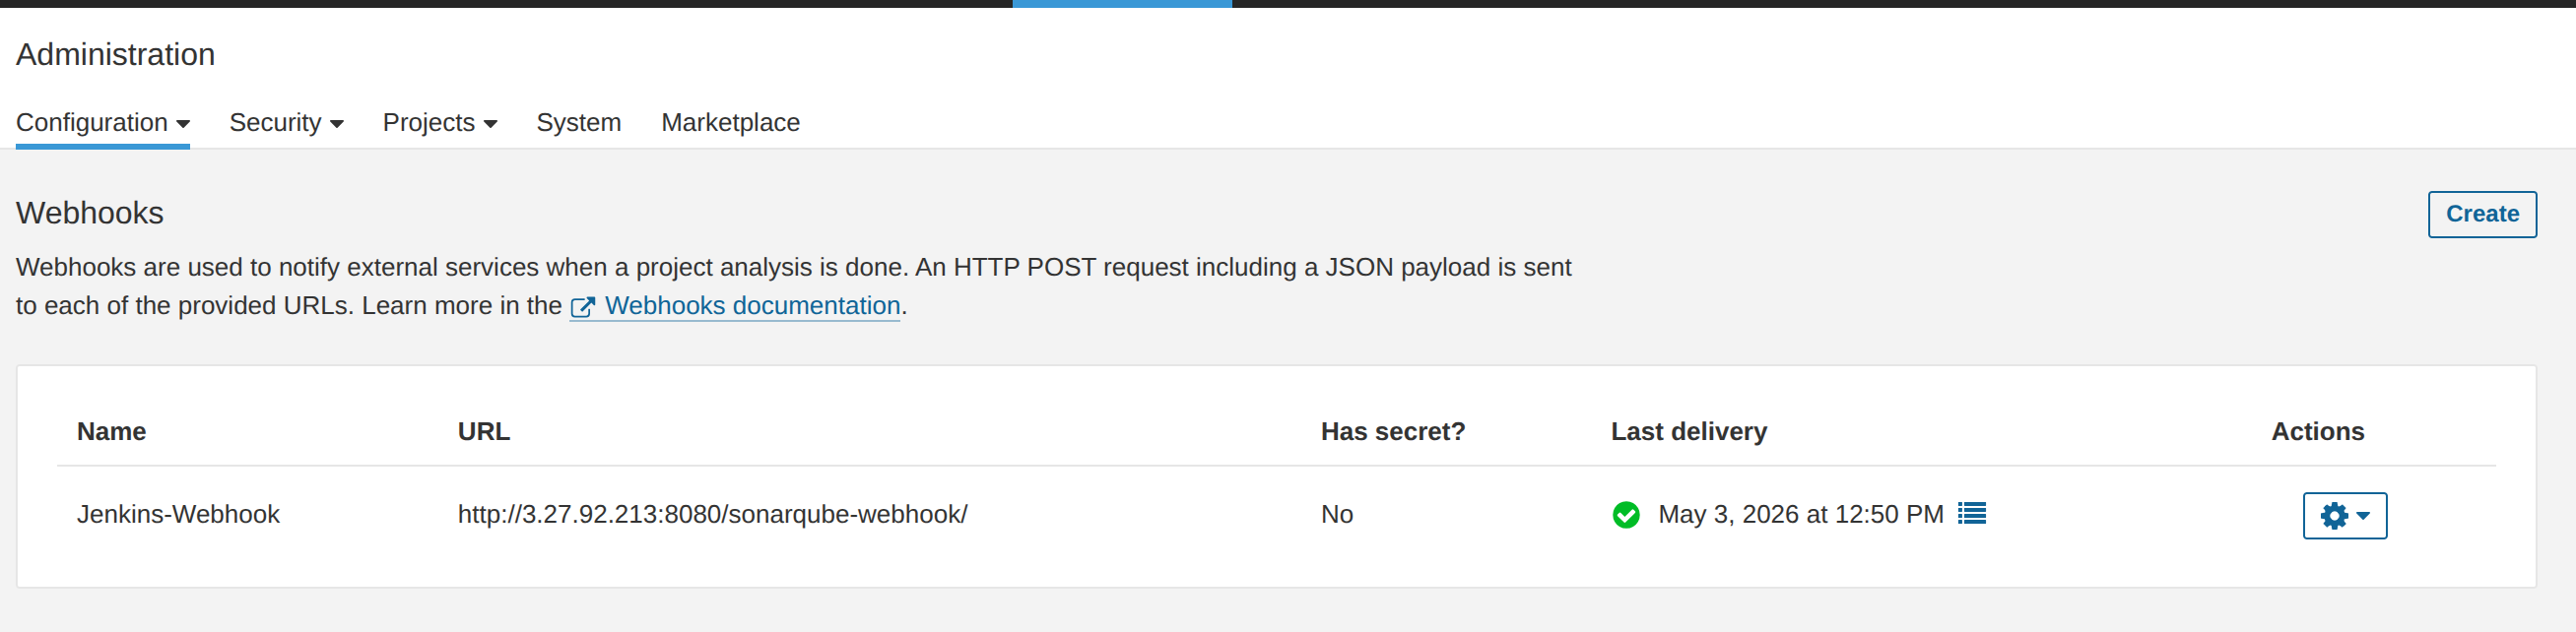
\includegraphics[width=0.9\textwidth]{img/06-sonarqube-webhook-config.png}
    \caption{Cấu hình Webhook gửi dữ liệu ngược từ SonarQube về lại Jenkins}
\end{figure}

\textbf{Quản lý thông tin bảo mật}: Thiết lập các ID Credentials trong Jenkins (\texttt{sonarqube-token}, \texttt{snyk-token}) để kết nối an toàn với các dịch vụ bên thứ ba.
